
\chapter{Limpieza de datos: extracción de usuarios relevantes}
\label{chap:extraccion_de_usuarios}

Como hemos visto en el análisis exploratorio inicial de los datos, la fase 
de limpieza de la información va a ser muy relevante para conseguir
nuestro objetivo final. Se trata de extraer, a partir de los tuits almacenados, 
una lista de usuarios que pudieran constituirse en candidatos adecuados a 
una oferta de trabajo (como, por ejemplo, las de la figura \ref{fig:ofertas_descripcion}). 
Para ello, de todos aquellos usuarios de los que tenemos constancia en 
los tuits recogidos hemos de seleccionar aquellos que sean personas (eliminando bots, 
empresas, etc.) y que hayan publicado contenido relacionado con la materia de referencia, 
en este caso la ciencia de datos.


Los desarrollos descritos en este capítulo están en el fichero {\bf seleccion\_usuarios.py}, 
que puede encontrarse en el repositorio de GitHub.

\section{Detección del idioma} 

El primer paso para poder analizar el contenido de un tuit y determinar si dicho tuit 
(y por tanto el usuario que lo ha publicado) está relacionado con la ciencia de datos o el big data,
es determinar el lenguaje en el que está escrito. Como ya hemos mencionado,
aunque la búsqueda en Twitter se realizó solicitando el campo \lq\lq languages = ["es"]\rq\rq,
obtenemos algunos tuits en otros idiomas, como estos dos 
que mostramos a continuación:

\myfigure{
\begin{tabular}{cc}

\includegraphics[width=0.4\textwidth]{tuit_ingles1}
&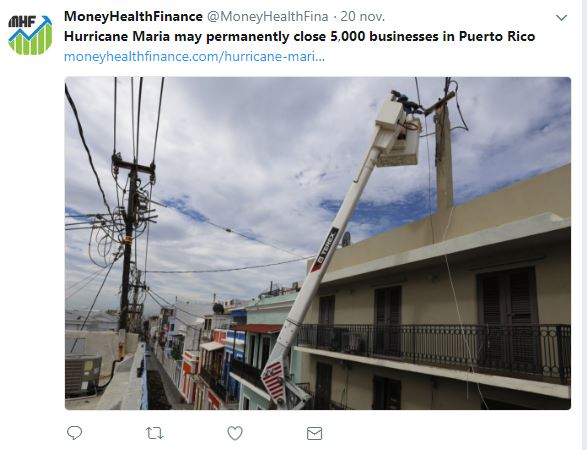
\includegraphics[width=0.4\textwidth]{tuit_ingles2}
\end{tabular}
\figcaption{Tuits no solo en español.}
\label{fig:tuits_ingles} }

Los primeros trabajos sobre el problema de la detección automática del lenguaje de un texto
se remontan a la década de 1970 \cite{zissman-berkling}. En la mayoría de las propuestas, 
existe una fase de entrenamiento, sobre textos previamente clasificados, en la que se produce 
un modelo del lenguaje (tal vez uno por lenguaje), y una fase de reconocimiento, en la que 
el lenguaje de mayor verosimilitud para el texto se extrae a partir de la aplicación de los 
distintos modelos. La clave de todos estos métodos es la modelización del lenguaje, algo que puede 
conseguirse atendiendo a diversas características diferenciadoras: fonemas, morfología, 
sintaxis y/o prosodia. 

La aplicación de dichas técnicas a textos provenientes de entornos web, blogs,  foros, etc. 
no está exenta de problemas, ver por ejemplo \cite{almeida_estevez_piad}.
Los textos procedentes de entornos web en general, y de Twitter en particular, 
presentan elevados niveles de lo que podríamos denominar como \lq\lq ruido\rq\rq,
por ejemplo:
\begin{itemize}
\item suelen ser textos cortos, lo que dificulta la aplicación de técnicas basadas en frecuencia 
de palabras o caracteres,
\item presencia de enlaces web, etiquetas, emoticonos y otros caracteres propios del entorno,
\item uso de jerga, lenguaje informal y palabras en idiomas distintos del principal del texto,
\item modificaciones de la ortografía, que van desde palabras abreviadas (\lq\lq q\rq\rq, 
\lq\lq xa\rq\rq) a expresiones enfáticas (\lq\lq mooooooolaaaaaaaa\rq\rq), por poner dos 
ejemplos.
\end{itemize}


A pesar de que es posible encontrar corpus de textos con estas características 
ya clasificados por 
idioma\footnote{\url{https://blog.twitter.com/engineering/en_us/a/2015/evaluating-language-identification-performance.html }}
que pudieran servir para entrenar un modelo que determinara el lenguaje,
hemos optado por usar un clasificador que no necesite entrenar un modelo, 
ya que esta parte del proyecto no es la principal. Hemos encontrado
referencias, como \cite{almeida_estevez_piad}, que apuntan al buen comportamiento de 
clasificadores que no depende de conjuntos de entrenamiento (basados en \lq\lq small words\rq\rq,
también denominadas \lq\lq stop words\rq\rq, y trigramas). Pero este método requiere de una implementación
{\em ad-hoc}, y las opciones disponibles, listas para usar, nos han parecido lo suficientemente
buenas para el objetivo que perseguimos en este apartado.


En el entorno de Python, hemos encontrado varios paquetes que tratan el 
problema de detectar el idioma de un texto automáticamente. Los más
comentados son los siguientes:
\begin{itemize} 
\item {\tt langid} \cite{langid}: es un paquete que proporciona un 
clasificador Naïve Bayes de textos, que usa $n$-gramas (secuencias de $n$ caracteres en el texto, con $1\leq n\leq 4$). 
El clasificador está pre-entrenado sobre diversos corpus de texto, en un total de 97 idiomas. Según los
resultados explicados en el artículo de presentación del trabajo, es un método con una
exactitud ({\em accuracy}) del 94\%.
\item {\tt langdetect}: de Nakatani Shuyo, también es un clasificador Naïve Bayes basado en $n$-gramas, con
normalizaciones heurísticas, \url{https://github.com/shuyo/language-detection }.
\item {\tt LDIG}: es un clasificador específico para Twitter, creado por el autor
de {\em lagdetect} para solventar las carencias de éste en la clasificación de mensajes
cortos, \url{https://github.com/shuyo/ldig }. Soporta menos idiomas que los anteriores.
\item {\tt equilid}: es el paquete de más reciente creación que hemos encontrado,
que además está especialmente diseñado para tratar el \lq\lq ruido\rq\rq
que comentábamos caracteriza los textos de Twitter. Está concebido para identificar
dialectos urbanos y tratar correctamente expresiones de jerga.
\end{itemize}

Dado el tema que nos ocupa, relacionado con ciencia de datos, la especialización 
de {\tt equilid} y la dificultad de su instalación en el sistema disponible
(usa una versión de TensorFlow que aparentemente no está desarrollada para Windows),
nos hace descartarlo de entrada. 
En \cite{langid2} se muestra que el comportamiento de cualquiera de los clasificadores 
restantes es lo suficientemente bueno por
separado para el objetivo de este proyecto. Sugieren que combinar dos o más clasificadores
puede mejorar la exactitud de la clasificación, y que en general, la limpieza de
los tuits (urls, etiquetas, menciones, etc.), si bien mínimamente en algunos casos,
suele mejorar el comportamiento de los modelos (excepto en el caso de {\tt langid}). 
Finalmente, nos hemos decidido por usar el algoritmo del paquete {\tt langid}, visto
el buen resultado reportado, y la facilidad de uso del mismo. 

En \cite{langid2} se muestra que, en un contexto general de detección del lenguaje, 
el paquete {\tt langid} no parece beneficiarse de una limpieza del tuit
para retirar urls, menciones, etiquetas y emoticonos del cuerpo del mensaje.
Sin embargo, dado que la implementación de esa limpieza no 
es difícil, hemos comparado la clasificación del lenguaje obtenido
con el texto original y con el texto limpio, y hemos observado que en los
textos de los $24,128$ tuits descargados (contando retuiteados y citados también)
hay un $6.37$\% de tuits que no tienen la misma asignación de lenguaje. 
Estos tuits suelen ser tuits con pocas palabras
o con mucha mezcla de idiomas (generalmente español e inglés).

Como método alternativo, se ha implementado un clasificador manual que solo
usa \lq\lq stop words\rq\rq para tratar esos casos en los que {\tt langid}
no da una elección clara del idioma. Si el método de los \lq\lq stop words\rq\rq
da un idioma para el texto que coincide con alguno de los proporcionados por 
{\tt langid} (bien el del texto limpio, bien el del texto original), ese será
el que se asigne al tuit. Y si no, lo dejaremos clasificado con un idioma desconocido.

Hemos aplicado este método de clasificación del lenguaje a los $24,128$ textos
de los tuits originales, retuiteados o citados, y resulta una clasificación en $25$
idiomas diferentes. Mostramos a continuación un resumen de los resultados del clasificador:


\myfigure{
\begin{tabular}{cc}
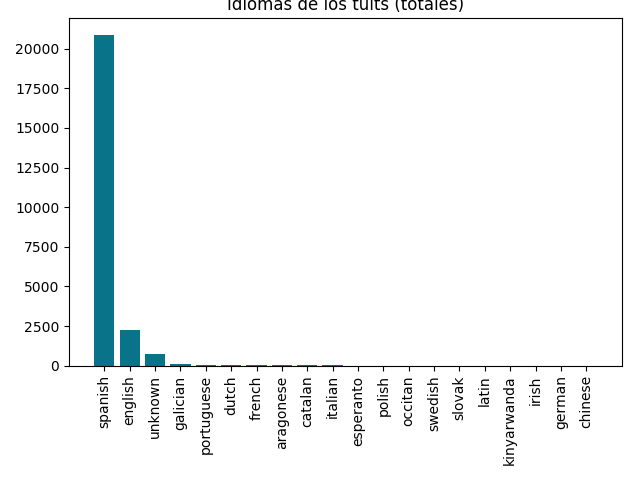
\includegraphics[width=0.4\textwidth]{C:/DATOS/MBIT/Proyecto/MBITProject_Data4all/Python/images/assigned_languages.png}
&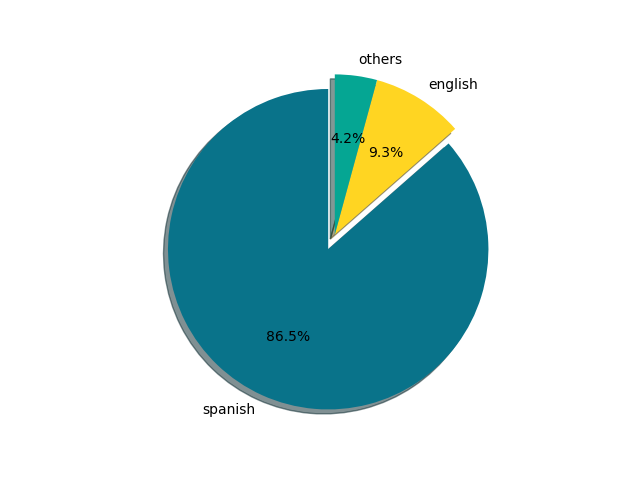
\includegraphics[width=0.4\textwidth]{C:/DATOS/MBIT/Proyecto/MBITProject_Data4all/Python/images/assigned_languages_proportions.png}
\end{tabular}
\figcaption{Clasificación por lenguaje del texto del tuit. Del $4.2$\% de \lq\lq others\rq\rq
hay un $2.9$\% de \lq\lq unknown\rq\rq. ¿Errores de clasificación?}
\label{fig:assigned_languages} }

Echando un vistazo a los resultados, aquellos que no están clasificados o que están
clasificados en idiomas poco probables, digamos, como el esperanto, son aquellos en los
que el clasificador seguramente ha fallado. Algunas veces parece ser porque casi no 
tuvieran texto o porque el texto contenga mucha mezcla de idiomas. Pero otras veces, 
como en el siguiente caso clasificado en esperanto, no está muy claro por qué:

\myfigure{
\begin{tabular}{cc}

\includegraphics[width=0.8\textwidth]{tuit_esperanto1}
\end{tabular}
\figcaption{Tuit clasificado como esperanto.}
\label{fig:tuit_esperanto1} }


\section{Tipo de usuario}
Para clasificar al usuario respecto a su entidad, y por ejemplo distinguir entre personas, bots y empresas, 
nos parece que la parte del tuit que más información contiene, a partir de los datos conseguidos, es
la bio que los propios usuarios aportan. Antes de cualquier labor de análisis de esos textos,
es necesario saber el idioma en el que están, y por ello de nuevo aplicamos a nuestros datos 
el identificador de lenguaje que usamos en el apartado anterior. 

Primero seleccionamos los datos correspondientes a los usuarios distintos, obteniendo
$7,210$ usuarios con distinto \lq\lq{\em id\_str}\rq\rq. {\tt langid} clasifica de 
forma diferente el idioma de los datos de perfil antes y después de 
limpiarlos (quitar urls, emojis, hashtags, etc.) en un $5.99$\%
de los casos. Después de aplicar en éstos últimos el método de las \lq\lq stop words\rq\rq, 
los perfiles de los usuarios han quedado clasificados en $44$ idiomas diferentes.

\myfigure{
\begin{tabular}{cc}
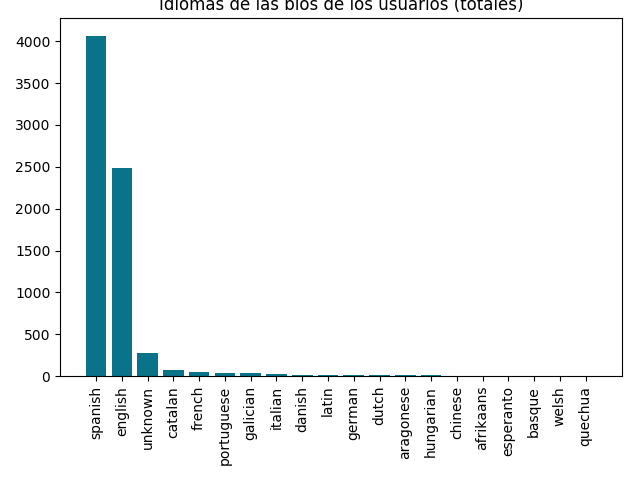
\includegraphics[width=0.4\textwidth]{C:/DATOS/MBIT/Proyecto/MBITProject_Data4all/Python/images/user_bios_assigned_languages.png}
&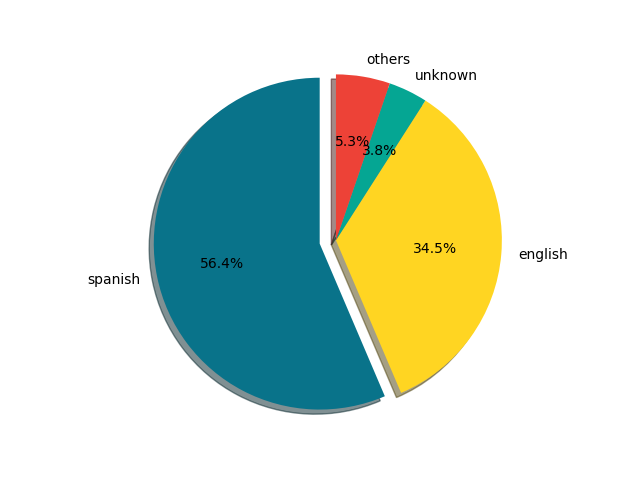
\includegraphics[width=0.4\textwidth]{C:/DATOS/MBIT/Proyecto/MBITProject_Data4all/Python/images/user_bios_assigned_languages_proportions.png}
\end{tabular}
\figcaption{Clasificación por lenguaje del texto de las bios.}
\label{fig:user_bios_assigned_languages} }


\section{Naturaleza del tuit}
texto del tuit:  IT, cientifico, analista o nodatascience (diccionarios de palabras)
					/Binario, data science o no data science
